\documentclass{lecturefig}
\begin{document}
\begin{frame}[fragile]
  \begin{tikzpicture}[
    C/.style={draw,circle,minimum size=1em},
    edge from parent/.style={draw,->},
    sibling distance=2cm,
    ]

    \node[C] (N) {N}
       child { node[C] (x) {x} }
       child { node[C] (y) {y} };

    \only<1>{
      \draw[dashed,->] (x) to[bend left]  node[above,sloped]{\scriptsize h} (N);
      \draw[dashed,->] (y) to[bend right] node[above,sloped]{\scriptsize h} (N);
    }

    \only<2>{
      \draw[dashed,->] (x) -- node[above,sloped]{\scriptsize h} (y);
      \draw[dashed,->] (N) to[bend left] node[above,sloped]{\scriptsize h} (y);
    }

    \only<3>{
      \draw[dashed,->] (x) to[bend left] node[above,sloped]{\scriptsize h} (y);
      \draw[dashed,->] (y) to[bend left] node[above,sloped]{\scriptsize h} (x);
    }

  \end{tikzpicture}
\end{frame}
\end{document}
